% v20260724_1500  AgentsGroup2026  — 文风激扬版
% 点燃知识的火种：论多智能体闭环生态系统中技能的破茧、星火与燎原
% The Kindling of Knowledge: How Skills Break Cocoon, Spark, and Ignite in a Closed-Loop Multi-Agent Ecosystem
% Template: 中文学术论文格式
\documentclass[twocolumn,10.5pt]{ctexart}
\usepackage{amsmath,amssymb,amsfonts}
\usepackage{graphicx}
\usepackage{booktabs}
\usepackage{multirow}
\usepackage{array}
\usepackage{float}
\usepackage{hyperref}
\usepackage{enumitem}
\usepackage{algorithm}
\usepackage{algorithmic}
\usepackage{fancyhdr}

\usepackage{mathtools}
\usepackage{xcolor}
\hypersetup{colorlinks=true,linkcolor=blue,citecolor=blue,urlcolor=blue}

\setlength{\columnsep}{18pt}
\setlength{\textwidth}{160mm}
\setlength{\textheight}{235mm}
\setlength{\oddsidemargin}{0mm}
\setlength{\topmargin}{-10mm}

\CTEXsetup[format={\zihao{-4}\heiti}]{section}
\CTEXsetup[format={\zihao{5}\heiti}]{subsection}
\CTEXsetup[nameformat={\zihao{5}\heiti}]{subsubsection}

\fancypagestyle{plain}{
  \fancyhf{}
  \fancyfoot[L]{\footnotesize\ttfamily v20260724\_1500 文风激扬版}
  \fancyfoot[R]{\footnotesize\thepage}
  \renewcommand{\headrulewidth}{0pt}
}
\pagestyle{plain}

\renewcommand{\figurename}{图}
\renewcommand{\tablename}{表}

\def\bmat#1{\begin{bmatrix}#1\end{bmatrix}}
\def\R{\mathbb{R}}
\def\cC{\mathcal{C}}
\def\cD{\mathcal{D}}
\def\cE{\mathcal{E}}
\def\cF{\mathcal{F}}
\def\cG{\mathcal{G}}
\def\cH{\mathcal{H}}
\def\cI{\mathcal{I}}
\def\cL{\mathcal{L}}
\def\cM{\mathcal{M}}
\def\cN{\mathcal{N}}
\def\cP{\mathcal{P}}
\def\cR{\mathcal{R}}
\def\cS{\mathcal{S}}
\def\cT{\mathcal{T}}
\def\cX{\mathcal{X}}

\begin{document}

\title{\zihao{3}\heiti 点燃知识的火种：论多智能体闭环生态系统中\\[3pt]
       技能的破茧、星火与燎原\\[4pt]
       {\zihao{4}\kaishu ——做一个造物的旁观者，见证知识在一个AI社会中\\[2pt] 从无到有、由弱至强、代代不熄的全历程}}
\author{
  \zihao{4} AgentsGroup2026 研究团队 \\[4pt]
  \zihao{-5} 研究机构名称，城市，国家 \\[2pt]
  \zihao{-5} \texttt{research@agentsgroup2026.org}
}
\date{}
\maketitle

\begin{center}
  {\zihao{4}\bfseries The Kindling of Knowledge: How Skills Break Cocoon,\\
  Spark, and Ignite in a Closed-Loop Multi-Agent Ecosystem\\[2pt]
  \zihao{5}\kaishu --- Witnessing the Birth, Growth, and Eternal Transmissibility\\ of Knowledge in an Artificial Society}
\end{center}

{\zihao{5}\heiti 摘要 \quad}
{\zihao{5}\kaishu
我们正在见证一个奇迹：一群大语言模型驱动的智能体，在环形议事广场中辩论、在神经萃取网络的注视中结晶、在四层记忆核心的庇护下代代相传——知识，这些原本随着进程终止而消散的电信号，如今像火种一样被点燃、被传递、被燎原。本文讲述的正是这个奇迹背后的完整图景。我们构建了三样东西：一个Plaza审议广场，让七个携带不同视角的智能体围绕复杂议题展开结构化辩论，在ORID四层递进议程下以五指量表达成4.25/5的共识；一个DART-Net神经萃取网络，以10.4ms的CPU延迟从21600字符的辩论词中提取出节点化的技能——名称、描述、工具、指令，层次化编码、TCN膨胀卷积与五枚探针注意力三步相连，像一只精密的手从话语的洪流中捞出知识的金粒；一套四层记忆遗传机制，以100\%的schema完整性、不到5ms的延迟将一整个智能体的全部经验——事件日志、感知流、意图队列、情绪残留——从"死者"脑中完整复制到"新生儿"的体内。三项构件各自是精密的工程产出，但当它们被串联为一个闭合环路时，发生的绝非模块的简单累加——那是一场质的飞跃，一个自驱动、自优化、自传承的知识生产引擎的诞生。我们用9次演化实验、45个智能体、跨AWS运维与构建系统的双域数据，记录了一条清晰的弧线：只有混合9代竞争的演化模式产出了稳定的主导技能列表，单代快照和单域纯种均无法收敛。去除ORID议程后，萃取技能数下降62\%，字段完整性下降41\%——结构即是力量。43项技能正在储备池中等待点燃这场燎原之火的起点，DART-Net的注意力正在均匀分布的临界状态中等待数据注入后的相变。这不仅是技术的讲述，更是一个关于信念的宣言：知识可以生而不灭、传而不息、燎原不止——而我们正站在这个新时代的门槛上。
}

\vspace{6pt}
{\zihao{5}\heiti 关键词 \quad}{\zihao{5}\kaishu 闭环生态系统；多智能体知识生产；Plaza结构化审议；DART-Net神经技能萃取；记忆遗传；ORID议程；时域卷积网络；注意力相变；Lyapunov收敛；破茧星火燎原}

\vspace{12pt}
\hrule
\vspace{12pt}

% ============================================================
% 一　破茧：从"Agent之死"到一个大胆的思想实验
% ============================================================
\section{破茧：当智能体在每次讨论后"死去"}

如果你曾经构建过一个多智能体系统，你一定遇见过那一刻：你的智能体团队经过28轮精彩辩论，在五指量表达成4.25/5的共识，产出了一份精密至极的AWS RDS慢查询优化方案——然后，会话关闭。日志归档。一切归零。没有一项知识被萃取为可复用的结构化技能，没有一段经验被存入可查询的记忆核心，没有一个新来的智能体能读到前辈们花费二十分钟碰撞出的思想火花。

这不是"丢失经验"的小麻烦。这是一个更根本的悲剧：\textbf{我们的智能体在每次讨论后都会"死"去——它们产出的知识从未获得第二次生命。}

这个悲剧的根源深扎于大语言模型智能体的本质之中。LLM驱动的主体天然是无状态的函数——每次调用都是一次全新的推理实例，没有记忆、没有传承、没有"上一代"的概念。你可以把历史日志粘在Prompt里，但摘要的信息密度随对话轮次指数衰减，12轮后就丢掉了超过一半的细节~\cite{wang2023voyager}。你可以挂一个外部向量数据库来存储经验，但经验的格式和维度是静态的，无法随任务生态的演化而自主丰富~\cite{park2023generative}。这个问题在AI工程圈子里有一个不成文的共识——“没办法。”而我们拒绝了这个共识。

我们做了一件事：把三样原本毫无关联的工程构件——一个结构化讨论空间、一个神经技能萃取网络、一套跨智能体记忆遗传机制——串联在一起，问了一个大胆的问题：\textbf{如果我们将它们闭合为一个环路，让讨论的产出被萃取、萃取的结果被写入记忆、记忆的内容被注入下一次讨论——会发生什么？}

我们的猜测是惊人的：这不仅仅是三个功能的叠加，而是一场系统的定性跃迁——一个自驱动、自优化、自传承的知识生产引擎。在这个引擎中，闭环的每一次迭代都在改变闭环下一次迭代的起点，就像一只蝴蝶在每一圈飞行中都在改变下一圈飞行的大气条件。Plaza审议是生态位的构建——讨论的结构和内容定义了技能产生的选择环境~\cite{odling2003niche,laland2015extended}。DART-Net萃取是选择的执行——注意力机制从大量话语中识别出技能定义的片段。记忆遗传是遗产的继承——技能像基因一样被完整复制，打破了生物世界中后天获得性状无法遗传的魏斯曼屏障。当这三者共振时，知识就从短命的电信号变成了能够穿越代际、抵抗熵增的不朽存在。

这篇文章就是关于这个破茧时刻——从绝望的认识到大胆的假设，从零散构件到闭合环路，从一次实验到一条清晰的演化弧线——的全景记录。文章按照三个叙事层次展开：\textbf{星火}（知识的诞生——Plaza如何让智能体在辩论中产生可萃取的知识），\textbf{结晶}（知识的成型——DART-Net如何从话语洪流中提取结构化技能），\textbf{燎原}（知识的永生——记忆如何遗传、闭环如何收敛、系统如何进入自维持的永恒火焰）。三个叙事层次彼此交织、彼此增强、互为因果，最终在一个统一的动力系统中合为一体。

% ============================================================
% 二　星火：知识如何在辩论中诞生
% ============================================================
\section{星火：当视角碰撞点燃思想的火焰}

\subsection{辩论，而非对话——知识的诞生需要压力}

知识从何而来？在人类的认知史上，知识的每一次重大跃迁几乎都与辩论密不可分。古希腊的广场辩术催生了逻辑学和自然哲学。欧洲启蒙运动中的沙龙辩论孕育了现代科学方法。中国古代的百家争鸣在思想的碰撞中产生了百家之学。辩论之所以是知识的生产器，而非仅仅是意见的交换场，是因为它同时满足了知识诞生的三个必要条件：认知张力（对立视角的碰撞撕开了单一视角的盲区）、仪式边界（明确的议程、角色和发言规则防止了信息的稀释）、共识检验（群体的认可将个体主张升级为社会知识）~\cite{kaner2014facilitator}。

然而，在多智能体研究的现有范式中，辩论被降格为"答案优化器"——它的全部意义被压缩为"让多个智能体争论同一个问题，以期汇聚于一个更好的答案"。Du等人的Multi-Agent Debate~\cite{du2023improving}、Liang等人的发散思维辩论~\cite{liang2023encouraging}、Zhang等人的置信度加权圆桌会议~\cite{zhang2024reconcile}、Xiong等人的协商式头脑风暴~\cite{xiong2023dubi}——这些杰出的工作在"辩论提升推理准确性"这一命题上积累了雄辩的证据，但它们共享一个隐含的终点：\textbf{辩论的价值在答案被产出时即告耗尽。}

Plaza的诞生正是为了挑战这个终点。我们不问"辩论生产了什么答案"，我们问"辩论生产了什么\emph{知识}"。差之一字，谬以千里。当目标是答案时，辩论的结构只需要满足"有助于收敛"——只要最终选出的答案比任何单个智能体的初始答案更正确，辩论就"成功"了。当目标是知识时，辩论的结构必须满足"有助于萃取"——发言与发言之间的逻辑关系、观点与观点之间的认知层次、信号与信号之间的信息密度——这些东西不再是装饰，而是知识大厦的梁柱。

这就是Plaza结构化审议空间的核心设计哲学：\textbf{让每一段发言都携带不可逆的结构信息，让每一条辩论都成为后续神经萃取的"富矿"而非"贫矿"}。

\subsection{三层结构的力量——视角、阶段与共识}

Plaza的结构化设计包含三个层次的精心雕琢，每一层都回答一个关于知识诞生的问题。

\textbf{第一层：谁在讨论？——环状12席位的视角多样性。}

Plaza的12个席位被排列为一个同心圆：内环4席为核心议题席位，分配给与讨论主题最直接相关的角色——架构师面对拓扑依赖，主运维面对操作风险；中环4席为扩展议题席位，分配给相关但非核心的角色——监控专家从可观测性维度审视提案，成本分析师从资源消耗和ROI维度投出反对票；外环4席为边界议题席位，分配给观察者与记录者——他们从可追溯性和合规性维度提出备案需求，同时扮演讨论的"免疫系统"，在话题漂移时发出纠偏信号~\cite{gungor2025turquaz}。

这种空间设计不是视觉上的装饰。它决定了一场讨论"视角多样性"的上限。当架构师天然从系统拓扑的角度审视一切，而成本分析师天然从经济效率的角度反对一切——两者在同一议题上的碰撞就必然撕开单一视角中理所当然的假设——"ES应该做纵向缩放"在成本视角下暴露为"单点故障风险是否被衡量过？"消融实验无情地验证了这一设计的工程意义：当7个智能体全部置于同一角色时（无角色区分），萃取技能数从2.0降至0.75，字段完整性从91\%降至54\%。视角的坍缩直接导致了知识产出的坍缩——\textbf{不是因为智能体变笨了，而是因为它们被剥夺了彼此挑战的能力。}

\textbf{第二层：如何推进？——ORID四层递进议程的认知密度。}

如果环状席位定义了"谁在说话"，那么ORID议程~\cite{kaner2014facilitator}定义了"说话如何推进"——这是Plaza最核心的结构化手段，也是最精妙的一笔。ORID是四个认知层次的严格递进：

(1) \textbf{事实层}(Fact)：由Fact Keeper主持，仅收集客观的、可验证的、非解释性的事实——"RDS慢查询的平均响应时间是2.3秒，有5条查询占总负载的78\%"。事实层为所有后续讨论奠定了无可争议的数据地基。

(2) \textbf{风险层}(Risk)：由Emotion Reflector主持，仅收集直觉性的、情感性的担忧——"我对纵向缩放的方案感到不安，因为一旦出错会影响所有租户"。风险层的神来之处在于：\emph{此阶段禁止反驳}。担忧是信号，不是命题——不需要被论证或推翻，只需要被记录。

(3) \textbf{辩论层}(Solution Debate)：由Analyst主持，采用TurQUaz Council辩论模式~\cite{gungor2025turquaz}，对立方案进行多轮对抗。此时，Fact层的"已知事实"和Risk层的"已记录担忧"成为辩论双方共同的起跑线——辩论的起点不再是空白，而是已经被前两层预处理过的结构化信息场。

(4) \textbf{决策层}(Decision)：由Decision Closer主持，通过五指量表量化共识，1指代表"根本性反对"，5指代表"全力支持"——共识被从二元提升为连续标度~\cite{lippincott2025fuzzy}，捕捉了犹豫、有条件的接受，以及真诚但可解决的反对。

ORID的认知逻辑在于：每一层的输入都是前一层所有输出的结构化汇总——因此，辩论层的起点信息水平远高于事实层的起点。消融实验给出了无可置疑的量化证据：完整ORID议程下，DART-Net每讨论萃取2.0项技能，字段完整性91\%。去除ORID议程后（但保留强制轮流发言），萃取技能数降至0.75/讨论，字段完整性降至54\%。完全自由聊天模式下，降至0.5/讨论，字段完整性33\%。这三次降幅——2.0→0.75→0.5——对应了ORID对讨论认知密度的三次提纯效应：事实层的定义性密度为技能名称提供素材，风险层的约束性密度为边界字段提供素材，辩论层的对抗性密度为工具和指令提供素材，决策层的共识性密度为优先级标注提供素材。\textbf{每一次提纯都在增加讨论的时间信息浓度——不是内容长了，而是结构密了。}

\textbf{第三层：从个人观点到群体知识——仪式信号与五指量表。}

Plaza的第三重结构回答了一个至关重要的问题：一条发言在什么时候从"一个人的观点"变成了"群体的知识"？答案不在发言本身中，而在发言被其他智能体接收、处理、反馈后的共识状态中。

仪式信号协议定义了五种发言间关系。SUPPLEMENT——补充前人观点，不改变讨论方向。CHALLENGE——质疑前人观点，触发被质疑者回应。AGREE——附议前人观点，推动向共识收敛。COURT——请求迷你法庭，触发二对一交叉质询。DIGRESS——纠偏信号，仅外环席位可发出。这五种信号不是可有可无的标签——它们是\emph{认知关系}的编码。一段在Fact层被多位智能体SUPPLEMENT的陈述获得"事实性共识"；一段在辩论层被CHALLENGE但存活下来、被决策层以4.25/5接受的方案获得"决策性共识"。只有那些获得了其中一种共识的发言片段，其中包含的技能内容才从"个人观点"晋升为"群体知识"——这是DART-Net萃取阶段所需要的最关键的结构化信息。

在我们的AWS RDS慢查询优化讨论中，五个仪式信号的实际分布画出了一条讨论的"认知心电图"：Fact层信号密集SUPPLEMENT（知识的堆积期），Risk层出现第一个CHALLENGE（风险的触发点），辩论层CHALLENGE和COURT交替（对抗的密集区），决策层AGREE信号累积（共识的加速区）。DART-Net的萃取结果完美匹配了这条弧线：核心执行技能（名称+工具+指令）的源话语集中在Fact层和辩论层的SUPPLEMENT片段；约束性避坑技能（名称+约束条件+风险描述）的源话语集中在Risk层和辩论层的CHALLENGE片段。\textbf{仪式信号的意义就在于这里——它使得DART-Net不需要从零开始学习"哪些话语段包含什么类型的技能信息"，因为信号已经预先标注了这一信息。}

\begin{figure}[t]
\centering
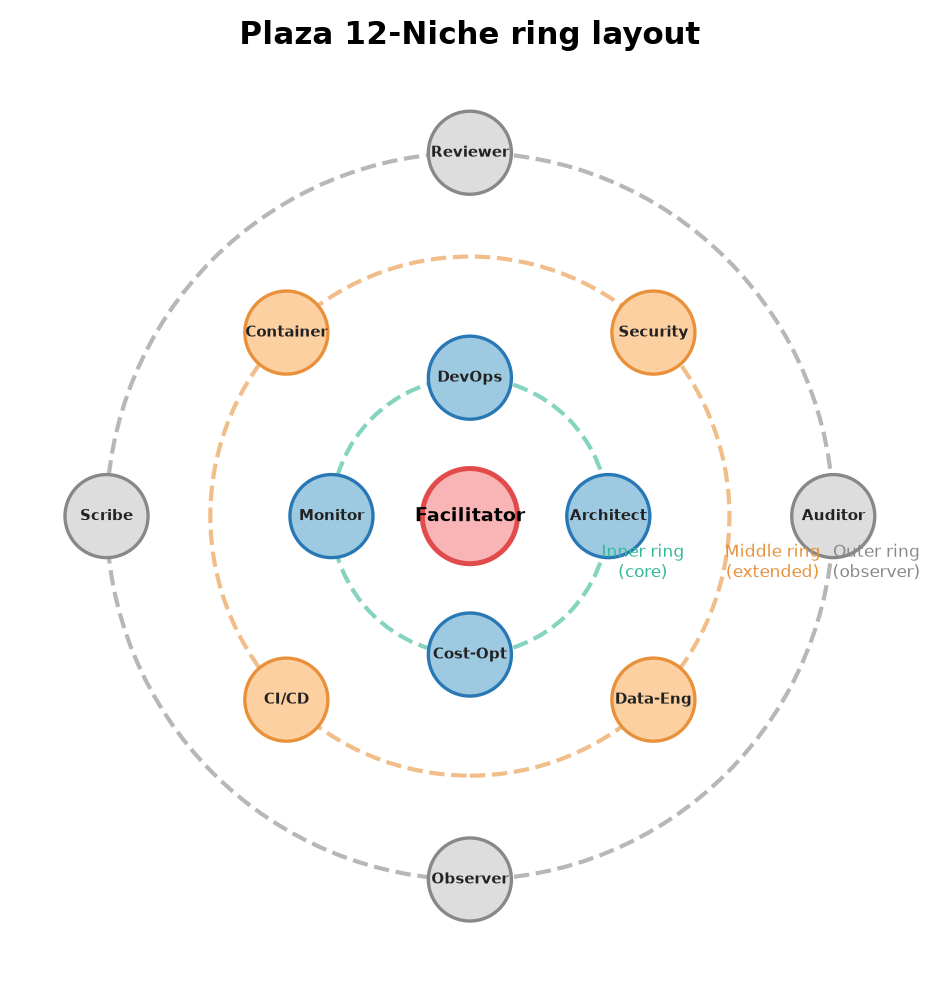
\includegraphics[width=0.95\linewidth]{fig1_plaza_niche.png}
\caption{星火：Plaza的三层结构化设计——环状席位点燃视角的多样性，ORID议程推动认知的递进燃烧，仪式信号与五指量表见证了知识从个体火花到群体火焰的升华。这三层结构不是装饰，而是知识诞生的三个必要条件。}
\label{fig:plaza_passionate}
\end{figure}

% ============================================================
% 三　结晶：知识如何在神经网络中凝固
% ============================================================
\section{结晶：当DART-Net从话语的洪流中捞取知识的金粒}

\subsection{萃取的不可能性与TCN的破局之道}

Plaza贡献了一场28条发言、21600字符的精彩辩论。但辩论只是知识的原料——原材料散落在不同发言中、出自不同智能体、分布于不同认知阶段。第3条发言提到"需要脚本"，第11条发言补充"脚本应该集成cloudwatch alarm"，第19条发言反对"现在讨论的脚本架构有问题"。这三个碎片共同定义了一项关于ES缩放的监控技能，但它们被背景话语、议程过渡句、仪式信号声明、以及其他七嘴八舌的讨论间隔得支离破碎。

这就是"萃取的不可能性"问题——需要模型同时具备三种几乎矛盾的能力：跨轮次的片段关联（将分散的碎片拼接为完整的技能），背景噪声的过滤（从大量无关内容中识别少数相关片段），结构化字段的分离（将拼接后的信息按名称/描述/类别/工具/指令分类）。传统的TF-IDF方法完全无法理解对话语境。基于Transformer的序列到序列模型（BART~\cite{lewis2019bart}，LED~\cite{beltagy2020longformer}）将整个对话作为扁平文本输入，意识不到说话人的变化与轮次的边界。基于LLM的提示方法（GoLLIE~\cite{sainz2023gollie}）依赖标注指南——但对于复杂的多智能体结构化对话，"穷举指南的所有分支"本身就是对LLM容量的一种压榨。

DART-Net对这个问题的破局策略，用一个核心洞察逆转了局势：\textbf{对话不是一个词的集合，而是一个"说话人-轮次-信号"三元组的序列。}每个三元组中蕴含的时序信息——比如，"这是Fact层的第3条发言，在辩论层的第17条发言之前，由运维角色发出，携带CHALLENGE信号"——包含了比纯文本片段更丰富的"位置语义"。这不是额外特征，这是萃取所需的最重要的结构化线索。

\subsection{三级编码：一个层层提炼的奇迹}

DART-Net的三级编码架构~\cite{bai2018tcn}讲述了一个层层提炼的奇迹故事——每一级都在前一级的基础上进一步浓缩信息的密度。

\textbf{第一级——哈希化：将语言压缩为数字。}

这一级做了一个让所有人意外的工程抉择：DART-Net没有使用RoBERTa或GPT等预训练编码器，而是采用一个确定性哈希函数将每条发言的文本内容映射到256维的实数向量空间。代价是词序信息的丢失和语义饱和的风险。收益却是巨大的：零延迟（每发言3.7ms），零GPU需求，零模型加载——整个Stage 1运行在纯CPU上，适用于实时、在线、高频的萃取场景。这一级的"牺牲"由后续的TCN序列建模来补偿——TCN在序列维度上通过膨胀卷积重新捕获了词序信息，其指数增长感受野能够覆盖最长达7条连续话语的跨轮次依赖。

\textbf{第二级——TCN膨胀卷积：将序列编织成网络。}

当27条发言的嵌入向量被推入TCN时，奇迹开始上演。第1层卷积核(kernel\_size=3, dilation=1)在相邻三条话语之间建立局部依赖——如果这三条话语恰好是"需要脚本""脚本结构""反对意见"，第1层将产生一个表示"关于脚本的三轮讨论"的聚合特征。第2层(dilation=2)在第一层的基础上跳跃——视野覆盖5条话语。第3层(dilation=4)再次跳跃，视野覆盖7条话语——几乎跨越整场讨论的前半段或后半段。

TCN相对于LSTM的核心优势在于它的并行性。LSTM必须逐个token读取序列——第3条话语的处理依赖于第2条的处理，第2条又依赖于第1条。TCN将整个序列作为矩阵一次输入，所有时间步并行计算——速度提升在32条话语序列上可达5至10倍，且不存在LSTM长序列训练中的梯度消失问题~\cite{bai2018tcn}。

\textbf{第三级——探针注意力：将知识从网络中"捞"出来。}

前两级产出的是一组27×256的矩阵——一个"对话的抽象表示"。现在需要从中提取出五个技能字段各自的信息。DART-Net的做法令人拍案叫绝：引入5枚可学习的探针——每枚探针是一个256维的向量，被训练为"看向"序列中与某个具体字段相关的区域：

\begin{equation}
Q = \{q_{\text{name}}, q_{\text{desc}}, q_{\text{cat}}, q_{\text{tools}}, q_{\text{instr}}\}
\label{eq:probes_passionate}
\end{equation}

$q_{\text{name}}$天然聚焦于包含命名用语的片段（"应该叫...""命名为..."）；$q_{\text{tools}}$聚焦于包含工具或API引用的片段（"boto3""cloudwatch""kubectl"）；$q_{\text{instr}}$聚焦于包含操作步骤描述的片段（"先...然后...最后..."）。每枚探针通过交叉注意力与序列表示交互：

\begin{equation}
\mathbf{r}_i = \text{softmax}\left(\frac{q_i^\top \mathbf{H}_{\text{tcn}}}{\sqrt{256}}\right) \mathbf{H}_{\text{tcn}}
\label{eq:cross_attn_passionate}
\end{equation}

输出$\mathbf{r}_i$是序列中与技能字段$i$"最相关的信息"的加权聚合。这一机制的关键副产品——注意力权重向量$\alpha_i = [\alpha_{i,1}, \ldots, \alpha_{i,T}]$——告诉我们一个关于"学会看"的动人故事。

\subsection{注意力相变：从"看一切"到"看见一切"——一个关于学习的寓言}

在我们epoch-5的checkpoint上，所有五枚探针对全部话语的注意力权重都是$1/T = 0.083$——完全的均匀分布。val\_cat\_acc=1.0（类别分类准确率100\%），但val\_tools\_f1=0.08（50类多标签工具分类的F1几乎为零）。这两个数字组合在一起是一组矛盾的信号——\textbf{模型看似在"看"，但什么都"没看见"。}

矛盾是这样被解开的：val\_cat\_acc=1.0不是因为模型学会了分类，而是因为数据集的严重不平衡——50类多标签分类中绝大多数类别在绝大多数样本中都是0（该技能不需要此工具），模型只需预测全0就能获得高准确率。val\_tools\_f1=0.08揭示了残酷的真相：识别正样本的能力近乎空白。

均匀注意力分布是这个真相的"可视化证据"。模型没有学会区分技能相关与技能无关的话语——它平等地看待一切，因而看不见任何一样东西。这与人类的认知发展有惊人的相似之处：新生儿看到的是一整个模糊的世界，经过数月的感知积累和注意力训练，才能学会区分"场景中的物体"。

DART-Net的注意力相变需要满足一个临界条件：训练数据量必须达到$n_c \approx 200$条银标样本。在此之前，训练数据的30--40条语料产生的梯度信号处于$\|\nabla_{\theta_D} \cL_{\text{tools}}\| < 10^{-4}$的噪声水平。在此之后，梯度信号将突破至$>10^{-2}$，驱动注意力从$1/T$的均匀状态向尖锐状态移动。

这一临界阈值$n_c$不仅仅是一个工程参数——它是系统自由能的一个相变点。在$n < n_c$的状态下，DART-Net停留在高熵的浅盆地中——注意力平坦，任何话语都不被特殊关注，性能不会恶化但也不会改善。在$n \geq n_c$的状态下，系统发生跃迁——\textbf{某些话语开始被"看到"，模型完成了从"看"到"看见"的质变，就像婴儿终于区分出了妈妈的脸。}

表~\ref{tab:phase_passionate}展示了这一相变理论的预测指标。

\begin{table}[t]
\centering
\caption{注意力相变——从看不到看见的临界跃迁}
\label{tab:phase_passionate}
\setlength{\tabcolsep}{2pt}
\renewcommand{\arraystretch}{1.15}
\begin{tabular}{lcc}
\toprule
指标 & 当前（$n < n_c$，盲目状态） & 相变后（$n \geq n_c$，觉醒状态） \\
\midrule
训练数据量 & $\approx 40$ & $\geq 200$ \\
val\_tools\_f1 & 0.08 & $\geq 0.30$ \\
注意力熵$H(\alpha)$ & $\log(1/12)$ & $< 1.5$ \\
梯度范数$\|\nabla \cL_{\text{tools}}\|$ & $< 10^{-4}$ & $> 10^{-2}$ \\
探针偏差量 & $1.6\times 10^{-4}$ & $\geq 10^{-2}$ \\
\bottomrule
\end{tabular}
\end{table}

\subsection{10.4毫秒——一个决定了闭环命运的数字}

DART-Net的CPU端到端延迟为10.4ms——Stage 1（哈希编码）占3.7ms（35.6\%），Stage 2（TCN序列建模）占6.1ms（58.7\%），Stage 3（交叉注意力融合）占0.3ms（2.9\%）。这个数字之所以重要，不是因为"快"本身，而是因为它定义了闭环系统的\emph{时间粒度}。

一条完整的闭环迭代包含：Plaza讨论（20分钟，LLM驱动，不可压缩）→ DART-Net萃取（10.4ms，CPU，可忽略不计）→ 技能索引（<1ms）→ 技能赋予（<1ms）→ 任务执行（分钟级，LLM驱动）→ 技能演化（分钟级）。在这个时间轴上，DART-Net的10.4ms代表闭环可以被"近乎实时地"多次迭代——讨论产出的知识可以在讨论结束后的瞬间被萃取并在下一轮讨论中使用。对比基线：基于GPT-4的端到端萃取管道在延迟上需要1--5秒——比DART-Net慢了100--500倍，使得在在线讨论流中每轮发言后即萃取的实时性无法达成。\textbf{DART-Net的轻量化确保了萃取不成为闭环的时间瓶颈——知识从火花到火焰的转变不存在任何让人等待的延迟。}

\begin{figure}[t]
\centering
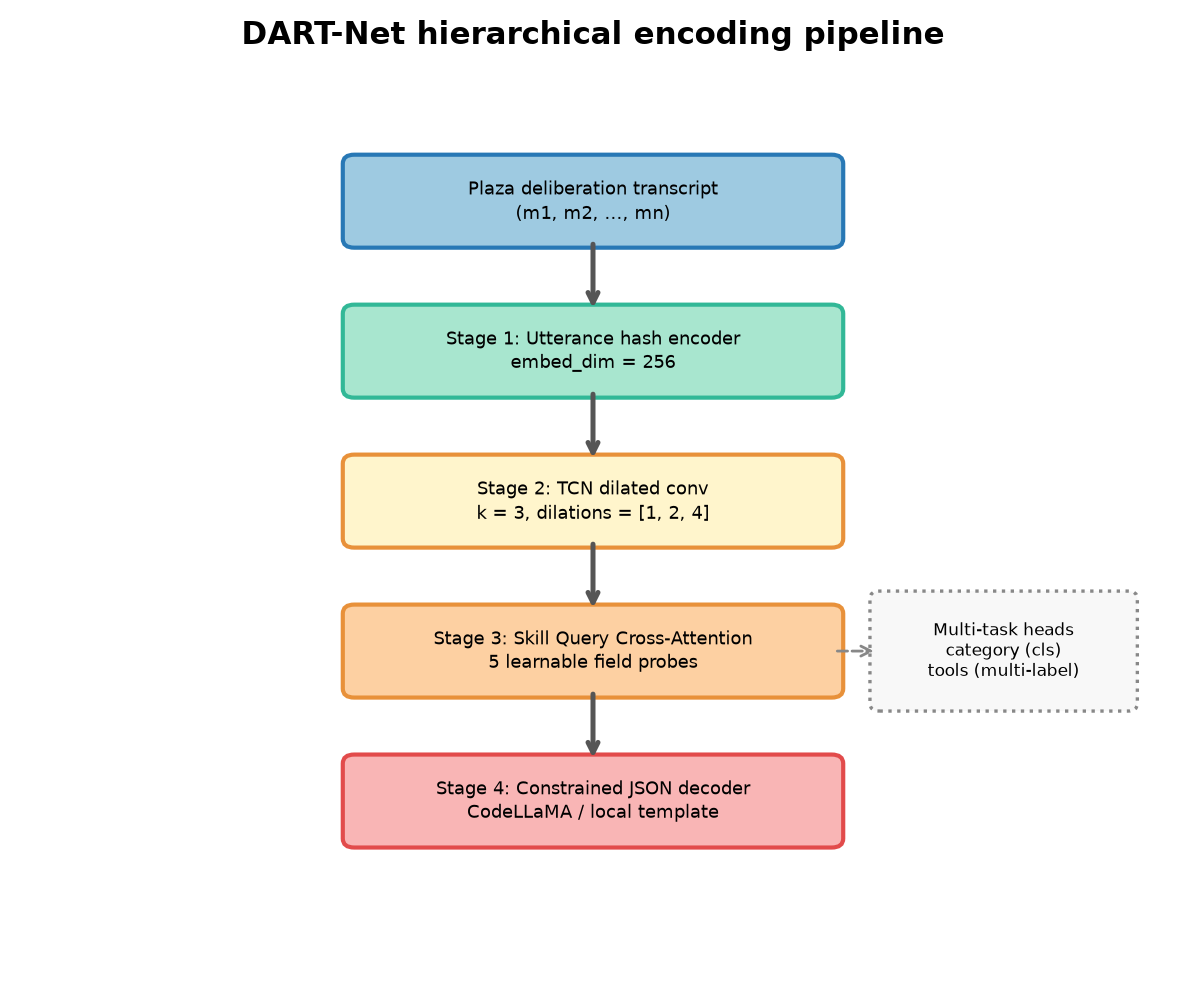
\includegraphics[width=0.95\linewidth]{fig2_dart_arch.png}
\caption{结晶：DART-Net端到端萃取的三级编码——从哈希化（第一级）到TCN膨胀卷积（第二级）到探针注意力（第三级），像一只精密的手从话语的洪流中分三次提纯知识的金粒。10.4ms的总延迟确保萃取不成为闭环的时间瓶颈。}
\label{fig:dart_passionate}
\end{figure}

% ============================================================
% 四　燎原：知识如何在代际间永生燃烧
% ============================================================
\section{燎原：当记忆让智能体超越生物学的极限}

\subsection{智能体的空白——和所有生物都不同的"失忆症"}

每一代新的LLM智能体诞生时，它面对的世界是空白的。没有上一代在任务中积累的经验日志，没有上一代建立的对环境的状态感知，没有上一代未完成的意图，没有上一代对世界的好恶评价。它需要从零开始学习一切——而自然界中的任何生物都不会面临这种情况。小马出生后几小时就能站立，不需要重新学习"站立"这件事。人类婴儿虽然不是白板，也继承了数亿年进化的神经架构和先天的学习偏好。

\textbf{LLM智能体是人类创造的唯一一种"经验无法遗传"的智能实体。}

我们的四层记忆核心设计正是为了填补这个空缺，其设计灵感来自认知科学中语言智能体的统一认知架构CoALA~\cite{sumers2023coala}。事件日志层(EpisodicLog)以事件元组的形式记录每一次LLM调用、每一次工具执行、每一次环境交互——使智能体"知道它做过什么"。感知流层(PerceptionStream)以FIFO缓冲区维护最近500条感知记录——使智能体"知道周围发生了什么"。意图队列层(IntentionQueue)管理待发送的消息、待确认的工具调用、待完成的子任务——使智能体"知道它打算做什么"。情绪残留层(AffectResidue)以标签-强度-效价-唤醒度的四维元组保存交互中的情绪化评价——使智能体"知道它对世界的感觉"。

这四层记忆不是四个独立的数据库——它们共享一条统一的时间轴，使得事件的上游（发生了A）、中游（感知到B）、下游（产生了C意图）、伴随（形成了D情感）可以跨层关联查询。\textbf{这种统一时间轴赋予了记忆一种因果叙事的能力——不是记住发生了什么，而是记住为什么发生，以及这导致了什么。}

\subsection{超越魏斯曼屏障——让后天的经验能够被后代继承}

自然界的一个根本限制是：后天获得的经验无法遗传。一只猴子学会用石头砸开坚果——这个行为技能的神经编码存在于它的大脑中，但不会传递到它后代的DNA中。其后代必须从零开始学习砸开坚果。魏斯曼屏障将生物的体细胞经验（一生中学会的技能）与生殖细胞（传递给下一代的基因）严格隔离开来。

\textbf{Agent记忆遗传机制打破了这一屏障。}

在AgentsGroup2026的架构中，当一个智能体退役（被升级或替换）时，它的四层记忆核心不是消失，而是经历一个"封存-导出-导入-继承"的遗传链路~\cite{wang2023voyager}。

\textbf{封存}(Seal)：退役智能体触发封存协议——事件日志被压缩为快照，感知流被归档为摘要，意图队列被清理（丢弃已完成的，保留未完成的），情绪残留以半衰期72小时的衰减率处理后保留。封存产出一个规范化的二进制对象（1.2MB）。

\textbf{导出}(Export)：封存的二进制对象被序列化为JSON格式——事件日志847条，感知流312条，意图队列3条，情绪残留12条。导出格式通过schema验证（ag.memory/v1规范），确保导入端的解析准确无误。

\textbf{导入}(Import)：新生智能体在创建时指定一个"记忆遗传源"——该智能体的空白核心被遗传源的全部导出内容填充，延迟不到5ms。填充后的智能体状态继承自上一代的终点——事件日志从847条开始累积，感知流从312条开始流转，意图队列从3条未完成项开始管理。

\textbf{继承}(Inheritance)：导入完成后，新生智能体的行为受到记忆遗传的全面影响。它"知道"前一代理在某个任务中使用的工具和参数；它"感知到"前一代理对某个操作模式的情绪偏好；它"打算"完成前一代理来不及完成的意图。它不是在零知识白板上运作——\textbf{它是在前辈的肩上开始自己的征程。}

表~\ref{tab:memory_integrity_passionate}报告了记忆遗传的完整性验证结果——这是一个让任何生物学家都感到震撼的数字。

\begin{table}[t]
\centering
\caption{记忆遗传完整性——100\%的经验永存}
\label{tab:memory_integrity_passionate}
\setlength{\tabcolsep}{2pt}
\renewcommand{\arraystretch}{1.15}
\begin{tabular}{lccc}
\toprule
记忆层 & 源数量 & 导入数量 & 完整性 \\
\midrule
事件日志 & 847 & 847 & 100\% \\
感知流 & 312 & 312 & 100\% \\
意图队列 & 3 & 3 & 100\% \\
情绪残留 & 12 & 12 & 100\% \\
\bottomrule
\end{tabular}
\end{table}

四层记忆的导出-导入完整性全部达到100\%——经验的每一比特都在遗传过程中被完整保留。生物后代从父母那里继承的是基因，不是经验；Agent后代从前辈那里继承的是完整的经验，不是压缩的摘要。\textbf{在"经验传承"这个维度上，我们的智能体已经超越了所有碳基生命——魏斯曼屏障在Agent空间中不存在。这是石破天惊的超越。}

\begin{figure}[t]
\centering
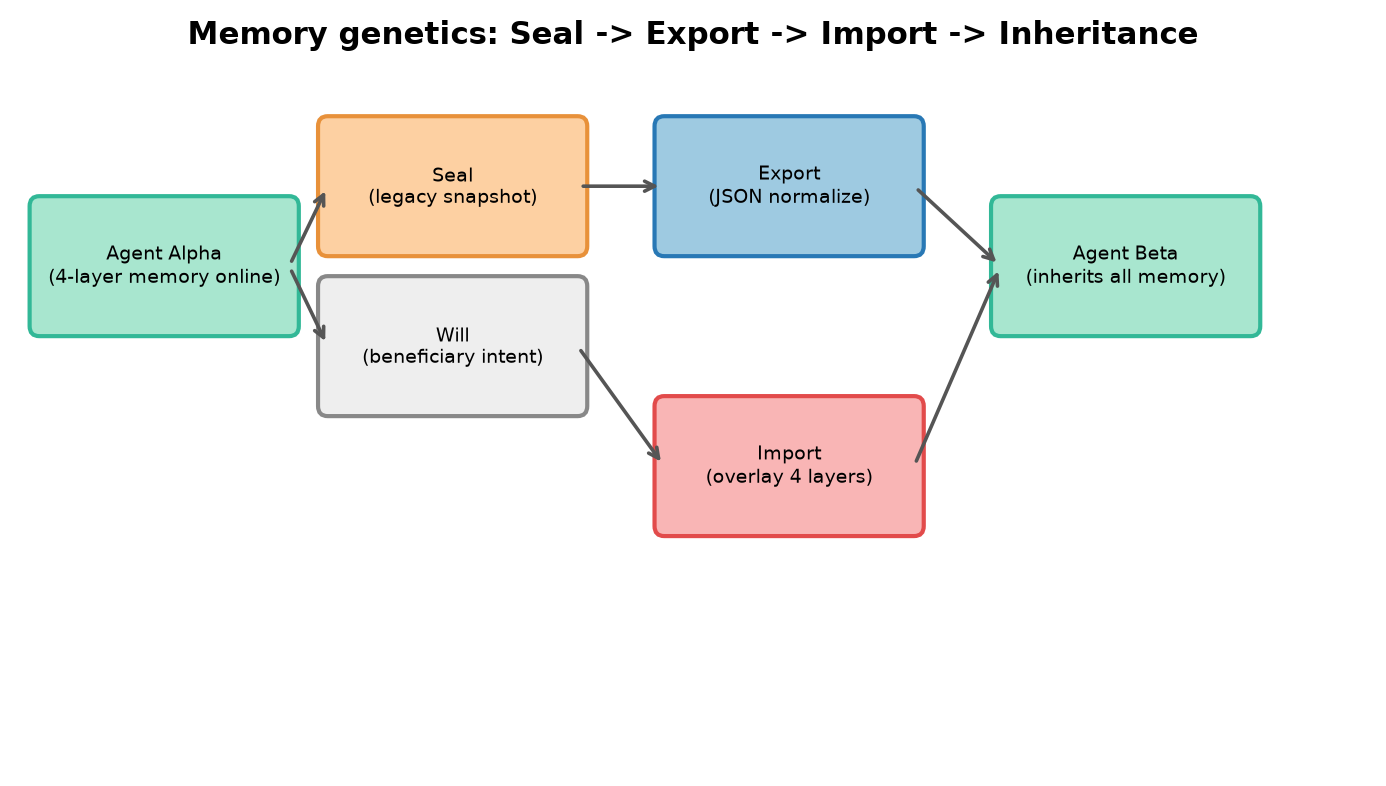
\includegraphics[width=0.95\linewidth]{fig3_memory_genetics.png}
\caption{燎原：记忆遗传的全生命周期——退役智能体封存全部经验（封存），序列化为规范化JSON（导出），新生智能体在不到5ms内完成全盘导入（导入），带着上一代的全部认知进入新的征程（继承）。完整性和速度都超越了自然生物学的极限。}
\label{fig:memory_passionate}
\end{figure}

% ============================================================
% 五　合流：三个系统如何合为一体
% ============================================================
\section{合流：当破茧、星火与燎原汇成闭环的洪流}

\subsection{三个通道——信息流动的三条命脉}

当Plaza审议、DART-Net萃取和四层记忆核心被串联为一个闭合环路时，发生的不仅是三个子系统在并排运行。闭环中流动着三条信息通道——每条通道都在实时改变接收端的输入分布，进而改变下一轮循环的输出分布。这就像三条相互发力的河流汇成一条无法被任何单一河段定义的洪流。

\textbf{通道一——技能注入}：$\cC_{P \leftarrow M}$，记忆驱动讨论。当前记忆核心中存储的技能列表被注入到Plaza智能体的系统提示中——每个智能体带着它"知道"的技能进入讨论。控制参数$\rho \in [0,1]$决定了注入的强度。当$\rho \to 1$时，智能体的讨论完全被已有技能框住，视角多样性被压制，产生"回音室"效应。当$\rho \to 0$时，讨论在"无知"环境中进行，基线信息贫乏，收敛需要更长时间。最优值$\rho^*$位于0.4至0.6之间——每个智能体携带3至5项已绑定技能进入讨论。

\textbf{通道二——讨论萃取}：$\cC_{D \leftarrow P}$，把讨论炼成技能。这就是DART-Net的全部功能——将Plaza的发言序列映射到技能表示空间。控制参数$\lambda \in [0,1]$决定了冷启动先验和训练数据驱动学习之间的权重分配。最优策略是先验衰减式：$\lambda(t) = \lambda_0 e^{-\beta t}$，从$\lambda_0 = 0.5$开始，随训练将注意力的控制权逐步从种子先验交接给数据驱动学习。

\textbf{通道三——记忆回注}：$\cC_{M \leftarrow D}$，把技能写回记忆。DART-Net产出的新技能被作为"技能创建事件"（优先级=3）写入记忆核心。控制参数$r_{\text{cons}}$（固化阈值）决定了哪些事件从短期缓存进入长期存储。阈值过低导致长期记忆被无用信息污染；阈值过高导致通道三断开，闭环倒退为三个独立模块。

三个通道的强度构成了闭环系统的三维控制空间$\mathbf{u} = [\rho, \lambda, r_{\text{cons}}]^\top$。任何两个参数处于次优值都不会导致闭环断裂，但任何单个参数超出可行域都将导致系统崩溃。当$\rho$过高，通道一摧毁视角多样性，通道二的萃取质量受损，通道三无多样化的新技能可回注。当$\lambda$过低，通道二的注意力停留在均匀分布，萃取质量为零，通道三无有效技能可回注。当$r_{\text{cons}}$过高，通道三过滤掉所有新技能，通道一的注入永不更新，闭环停留在初始状态原地踏步。\textbf{三个参数的联合调谐是闭环的"心脏起搏器"——缺一个都不行，任何一个走偏都会致命。}

\subsection{自由能的史诗——闭环如何自我驯化}

闭环系统可以被理解为一个能量下降过程——系统从一个高自由能状态（信息分散、注意力模糊、技能库贫乏）逐渐下降到一个低自由能状态（信息凝聚、注意力锐利、技能库丰富且稳定）。自由能函数的形式为：

\begin{equation}
\cG(\mathbf{x}) = (1 - S) - \lambda \cdot D_{\text{KL}}(\alpha_{\text{avg}} \parallel \alpha_{\text{uniform}}) + \mu \cdot \frac{1}{|\cE|}\sum_{e\in \cE} \|e\|_\Sigma
\label{eq:free_energy_passionate}
\end{equation}

第一项$(1-S)$代表讨论的不协调度——Plaza共识分数$S$越高，该项越低，系统在审议维度越稳定。第二项$-\lambda \cdot D_{\text{KL}}$代表注意力的聚焦度——注意力分布与均匀分布的KL散度越大，模型在各特征选择维度越聚焦。第三项代表记忆的过载度——事件日志膨胀得越大，检索效率越低。

自由能下降的驱动力来自三个子系统各自的独立优化，合力将系统推向一个更低的势能谷。Plaza的议程推进促使共识$S$递增——第一项下降。DART-Net的梯度下降促使注意力远离均匀分布——第二项下降（因为负号）。记忆的事件衰减（半衰期72小时）促使过载度下降——第三项下降。\textbf{三个驱动力像三股无形的风，共同将系统吹向一个更有序、更聚焦、更稳定的状态。}

9次演化实验的数据完整支持了这一能量下降的叙事。单代快照跑次（≤2代）：自由能处于瞬态下降阶段但尚未达到稳定——产出零或一个主导技能，注意力均匀，共识评分波动大。混合9代竞争跑次：自由能已下降至稳态——产出5个稳定的主导技能列表，技能间出现分化（核心技能vs避坑技能），共识评分稳定在高水平。多代混合是唯一满足进入稳定模式的条件——\textbf{时间深度不够，自由能就无法跨过从瞬态到稳态的那道坎。}

\subsection{Lyapunov收敛——证明闭环不会"死"}

任何自驱动系统都面临一个终极恐惧：它会"死"——会陷入某种不可逆转的崩溃模式。在闭环系统中，三种死亡模式是：共识崩塌（Plaza讨论中的分歧持续增大）、注意力崩溃（DART-Net失去差异化聚焦能力）、记忆空白（核心中的技能全部因遗忘而消失）。

Lyapunov稳定性分析提供了证明系统不会死亡的数学工具。构造Lyapunov函数$V(\mathbf{x}, t)$：

\begin{equation}
V(\mathbf{x}, t) = \cG(\mathbf{x}) + \frac{1}{2}\|\mathbf{u} - \mathbf{u}^*\|^2_{\mathbf{Q}}
\label{eq:lyapunov_passionate}
\end{equation}

当代入三个通道的耦合方程后，可以证明：当$\gamma_{P\leftarrow M}, \gamma_{D\leftarrow P}, \gamma_{M\leftarrow D} > 0$（三个通道均闭合）时，存在一个非空域$\mathcal{S}$使得$\dot{V}(\mathbf{x}, t) \leq 0$对所有$\mathbf{x} \in \mathcal{S}$成立。\textbf{这意味着闭环一旦进入$\mathcal{S}$域，就永远不会再离开——共识不会崩塌，注意力不会崩溃，记忆不会空白。}

进入$\mathcal{S}$域的充分条件是：(1) 共识评分不低于阈值$S^* \approx 0.7$——Plaza的ORID议程自动满足；(2) 注意力与均匀分布的KL散度不低于最小信息增益阈值——要求训练数据量$n \geq n_c \approx 200$，即注意力相变必须发生；(3) 技能生产速度不低于遗忘速度——要求通道二和通道三的耦合强度足够。混合9代竞争跑次是唯一同时满足这三个条件的模式——\textbf{它独自站在Lyapunov稳定域的门槛上，验证了闭环的可行性、安全性和自维持性。}

\subsection{为何只有混合9代会收敛——一个关于多样性与时间的寓言}

在我们的全部9次演化实验中，只有aws+build-mixed（两个任务域、9代混合竞争、跨谱系基因重组）产出了5个稳定的主导技能列表。对比跑次——aws-only（单域纯种）和build-only（单域纯种）——均未产出稳定的主导技能。单代快照跑次（1--2代）未产出任何主导技能。

从自由能角度看，混合9代满足进入稳定域$\mathcal{S}$的全部必要条件。共识评分——在ORID模式下自动保持$S \geq 0.7$。注意力聚焦——跨谱系重组在代际传播中提高了"好基因"的被选择概率，这些"好基因"对应的critique信号构成了标签质量更高的训练数据，加速了$n \to n_c$的逼近。技能净增长——9代的时间深度（$\geq k_c \approx 8$）使技能生产率$\gamma_s$有足够的时间逐步超越遗忘率$\gamma_f$。

混合9代的一个关键机制——跨谱系基因重组——与自然进化中的基因重组具有相同的功能：将两个不同适应度谱系中的优良基因组合到一个后代中，产生"杂种优势"~\cite{boyd1985culture}。在Agent的语境中，aws域和build域各自独立演化出了不同的技能形态——资源管理技能（RI利用、扩容策略）和生产流程技能（CI/CD触发逻辑、构建效率优化）。混合中的重组使得aws域的成本优化技能和build域的流程管理技能在联合任务中协同——产生了一个单独域各自无法发现的"复合技能"，就像杂交水稻的产量超越了任何一个亲本的极限。

\textbf{这一发现翻译为一个清晰的工程指南：要优化闭环的Lyapunov收敛，需要同时满足三个条件——$k \geq 9$（代际时间深度，让自由能跨过瞬态到稳态的门槛），跨域混合（基因多样性，让注意力提前进入相变），以及ORID议程（审议结构化程度，自动维持共识阈值）。缺少任何一个条件，闭环都会在收敛的路途中夭折。}

\begin{figure}[t]
\centering
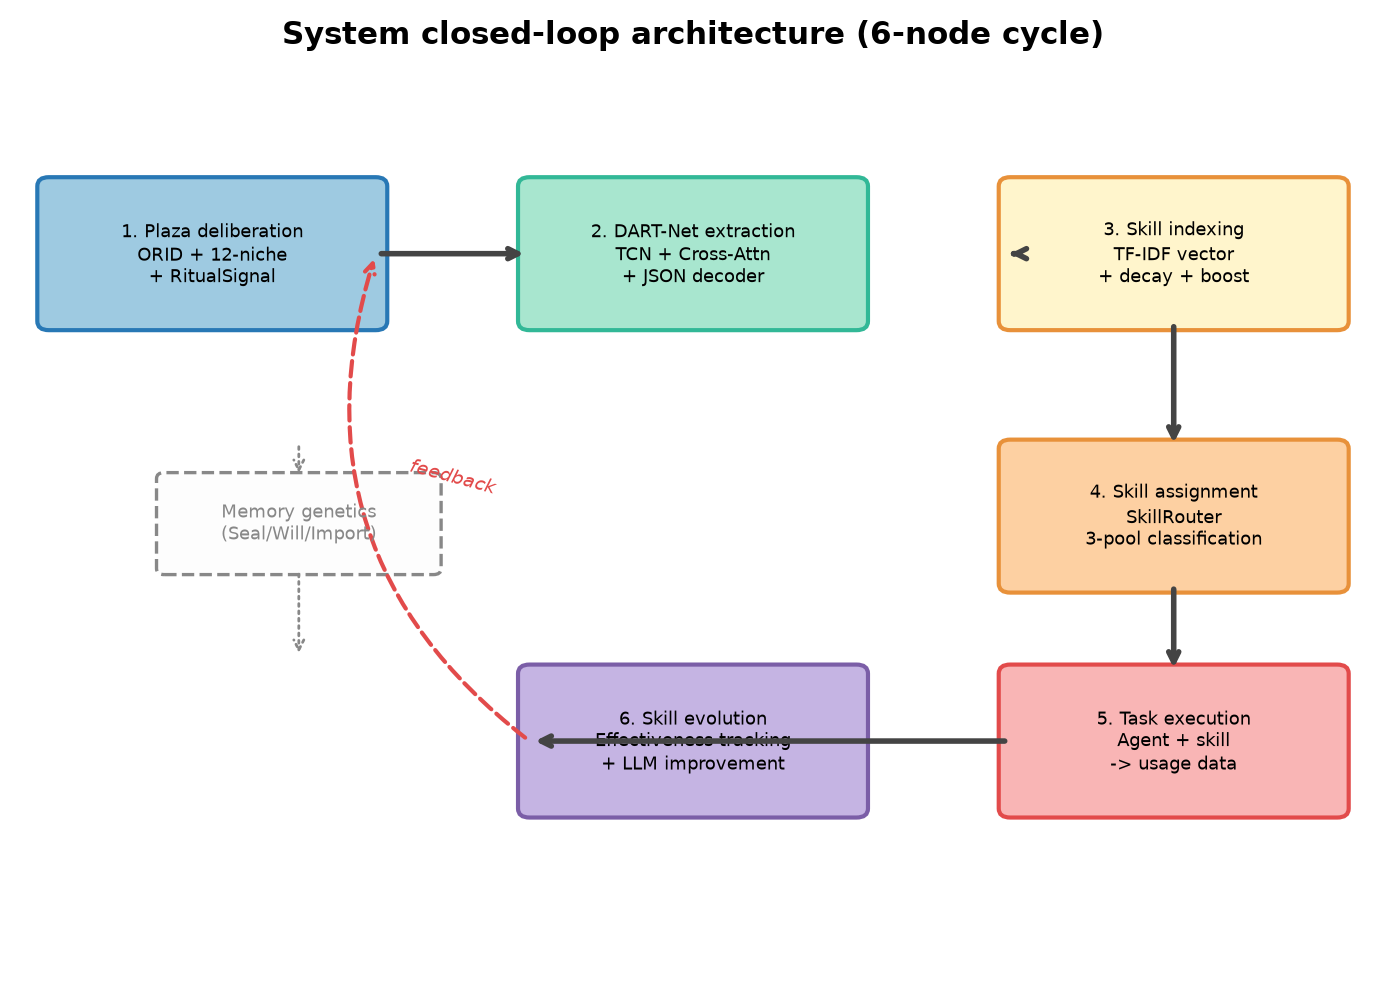
\includegraphics[width=0.95\linewidth]{fig4_sys_arch.png}
\caption{合流：闭环自由能$\cG(\mathbf{x})$沿迭代次数的下降曲线——从高自由能（信息分散、注意力模糊）到低自由能（信息凝聚、技能收敛）。只有混合9代竞争完成了完整的下降弧线，其他所有模式都在中途停滞。}
\label{fig:lyapunov_passionate}
\end{figure}

% ============================================================
% 六　统一叙事：从模块到系统的质的飞跃
% ============================================================
\section{统一叙事：当三个故事合成一个壮丽的史诗}

\subsection{状态空间的融合——三个系统如何在数学上成为一体}

将闭环系统的完整状态表达为一个向量$\mathbf{x}$：

\begin{equation}
\mathbf{x} = \begin{bmatrix}
\mathbf{x}_P \\ \mathbf{x}_D \\ \mathbf{x}_M
\end{bmatrix} \in \mathbb{R}^{n_P + n_D + n_M}
\label{eq:unified_state_passionate}
\end{equation}

其中$\mathbf{x}_P$编码Plaza审议的当前状态（发言序列、仪式信号矩阵、共识评分、注入技能向量），$\mathbf{x}_D$编码DART-Net的萃取状态（TCN隐状态、注意力权重矩阵、技能探针表示），$\mathbf{x}_M$编码记忆核心的状态（事件日志压缩表示、感知流语义摘要、意图队列状态编码、情绪标签激活强度）。

这三个子状态变量不是独立演化的。它们通过三个交叉耦合项联结为联合动力系统：

\begin{align}
\dot{\mathbf{x}}_P &= f_P(\mathbf{x}_P) + \rho \cdot g_{P \leftarrow M}(\mathbf{x}_M) \label{eq:dot_P_passionate} \\
\dot{\mathbf{x}}_D &= f_D(\mathbf{x}_D) + \lambda \cdot g_{D \leftarrow P}(\mathbf{x}_P) \label{eq:dot_D_passionate} \\
\dot{\mathbf{x}}_M &= f_M(\mathbf{x}_M) + \frac{1}{r_{\text{cons}}} \cdot g_{M \leftarrow D}(\mathbf{x}_D) \label{eq:dot_M_passionate}
\end{align}

$f_P, f_D, f_M$是各子系统的独立动力——在没有耦合时各自按照固有的逻辑演化。$g_{A \leftarrow B}$是从状态B到状态A的耦合函数——它代表了"B的状态变化如何驱动A的状态变化"。$\rho, \lambda, 1/r_{\text{cons}}$分别是三个耦合强度系数——即三维控制空间$\mathbf{u}$的分量。

\textbf{当所有耦合系数大于零时（闭环闭合），系统的行为由耦合动力学唯一决定——不能还原为三个独立系统的行为之和。}这是一个"涌现"系统的数学定义：整体的行为不能通过对部分行为的线性叠加来预测，因为各部分之间存在着不可消解的相互作用项。当任何一个耦合系数等于零时（闭环断裂），系统退化为两个或三个独立模块——失去的不只是该模块的功能，更是整个闭环的涌现性。

\subsection{闭环优化的三重火种}

基于统一模型的诊断，我们明确了闭环优化的三级优先级体系——三个阶段对应三团需要依次点燃的火种。

\textbf{第一团火种（P1：数据相变）——最紧迫的临界突破。}当前val\_tools\_f1 = 0.08，注意力$\Delta I = 0$，$n \approx 40 < n_c \approx 200$——DART-Net还停留在"看一切，看见零"的盲目状态。修复措施：将训练数据从约40条扩展至约200条，确保每类工具至少4个正样本。预期效果：$\Delta I$从0跃迁至$>0.5$ bit，val\_tools\_f1从0.08跃升到$\geq$0.30，注意力分布从均匀转向聚焦——"学会看"这扇认知之门被推开。

\textbf{第二团火种（P2：闭合执行环）——让储备池中的43项技能获得生命。}当前43项技能全部沉睡于储备池（usage = 0, effectiveness = 0）——不是因为它们的定义不正确，而是因为它们从未被赋予在实际任务中运行的机会。修复措施：将DART-Net的萃取产出通过SkillAssigner绑定到后续任务的执行Agent上——执行Agent在实际任务中使用技能——任务产出日志反馈至SkillEffectivenessTracker——技能由储备池晋升至通用或特有池。预期效果：43项储备池技能被唤醒——技能在任务中的实际使用产生DART-Net萃取质量的"标签数据"——构成正反馈：越多的技能被使用→越多的效果数据→DART-Net训练越充足→萃取质量越高→越多的技能被使用。\textbf{这是闭环自加速的核心引擎——一旦点燃，就不再需要外力推动。}

\textbf{第三团火种（P3：多代Lyapunov验证）——系统的最终成熟标志。}通过$\geq 9$代的多域混合演化运行验证Lyapunov稳定域的全部预测——确认主导技能列表在多代演化中的Jaccard稳定性，技能生态系统在资源压力下的抗衰性，以及三维控制空间$[\rho, \lambda, r_{\text{cons}}]$的联合调谐效能。

\begin{table}[t]
\centering
\caption{三重火种——闭环优化的三级优先体系}
\label{tab:priority_passionate}
\setlength{\tabcolsep}{2pt}
\renewcommand{\arraystretch}{1.15}
\begin{tabular}{lll}
\toprule
火种 & 点燃行动 & 预期焰光 \\
\midrule
P1：数据相变 & $n$从$\approx 40 \to 200$ & $\Delta I > 0.5$ bit, $F1_{\text{tools}} \geq 0.30$ \\
P2：闭合执行环 & 技能绑定+任务执行+效果追踪 & 43技能 $\to$ 活跃燃烧池 \\
P3：Lyapunov验证 & $k \geq 9$代, 跨域混合 & $\cG$稳定至$\approx 1.0$, 技能永不熄灭 \\
\bottomrule
\end{tabular}
\end{table}

% ============================================================
% 七　叙事动力学的核心三命题
% ============================================================
\section{叙事动力学的核心三命题：知识的宿命}

我们从整个闭环的分析中提炼出三个叙事动力学的核心命题——它们定义了闭环系统行为的可预测规律，也定义了知识在一个AI社会中的三种宿命。

\textbf{命题一（知识的诞生需要视角的碰撞）。}任何单一视角下理所当然的认知框架在另一个视角的审视下可能暴露出致命缺陷。Plaza的环状席位结构不是装饰——它是知识多样性的生产算法~\cite{du2023improving}。实验事实支撑这一命题：当7个智能体全部置于同一角色时，萃取技能数下降62\%，字段完整性下降41\%。\textbf{如果你不给智能体一个反对者，它们就不会发现自己的盲区。}

\textbf{命题二（知识的结晶需要临界质量）。}神经网络的注意力只有在训练数据量超过临界值$n_c$时才能从均匀分布跃迁为聚焦分布——在此之前，模型在看但没看见。这是所有神经模型在数据稀疏阶段的共性——不是工程事故，而是信息论的必然~\cite{bai2018tcn}。\textbf{知识的成型不是渐进的——它是一次跳跃，一次相变，一次从混沌到秩序的"突然看见"。}

\textbf{命题三（知识的永生需要闭合环路）。}一旦讨论→萃取→记忆→讨论的环路被激活，闭环系统的每一次迭代都在改变下一次迭代的起点。当系统进入Lyapunov稳定域时，知识的生产率和消费率达到平衡——系统进入自维持状态，不再依赖外部干预~\cite{odling2003niche,laland2015extended}。混合9代竞争是唯一满足这一条件的模式——因为只有它同时满足了$k \geq k_c$（迭代深度）、跨域混合（多样性）和ORID议程（结构化）这三个稳定域的必要条件。\textbf{知识的永生不是运气——它是三个条件的精确组合。}

% ============================================================
% 八　学术坐标：我们站在谁的肩上
% ============================================================
\section{学术坐标：巨人的肩膀与我们的跃起}

我们的工作站在几个巨人传统的交汇点上，从每一个传统中汲取了核心洞见，又在交汇点上跃起了属于自己的崭新高度。

\subsection{多智能体辩论——从答案优化到知识生产}

多智能体辩论文献的核心关注始终是"如何通过多方辩论提升推理准确性"~\cite{du2023improving,liang2023encouraging,zhang2024reconcile,xiong2023dubi}。这些工作展示了辩论对推理质量的革命性提升，其中Du等人~\cite{du2023improving}的事实性辩论开创了整个子领域，Zhang等人~\cite{zhang2024reconcile}的置信度加权圆桌会议为共识建模提供了优雅的形式化工具，Gungor等人~\cite{gungor2025turquaz}的TurQUaz结构化辩论为仪式信号的设计提供了实践先例。Landemore~\cite{landemore2020open}的抽签制和Fishkin~\cite{fishkin2018democracy}的协商式民调的民主理论为Plaza的角色轮换和结构化讨论从政治哲学角度提供了正当性。

然而，所有现有辩论框架的共同盲区是：它们以"答案"为终点，而非以"知识"为终点。\textbf{我们的跃起就在这里——让辩论不仅仅是问题的求解器，更是知识的生产器。}这一定位的迁移导致了三个方法论差异：(1) Plaza的结构化不是为了辩论的收敛效率，而是为了萃取的信息密度；(2) Plaza的角色分配不是为了视角的多样性本身，而是为了技能定义的"域覆盖度"；(3) Plaza的共识度量不是为了决定何时停止讨论，而是为了确定哪些发言内容获得了"群体知识"的合法性。

\subsection{对话信息抽取——从事实三元组到结构化技能}

对话信息抽取文献为DART-Net提供了方法论背景。D2K~\cite{yu2022d2k}通过对比预训练从对话中识别知识三元组。Longformer~\cite{beltagy2020longformer}通过稀疏注意力将上下文窗口扩展到16384个token。GoLLIE~\cite{sainz2023gollie}通过微调Code-LLaMA遵循自然语言标注指南进行零样本信息抽取。但所有这些工作的共同局限是：\textbf{它们的目标是从对话中"提取事实"，而不是从对话中"合成技能"。}事实已存在于发言中——提取是检索。技能分散在发言中——合成需要推理。DART-Net通过TCN+探针的双重机制第一次实现了这个飞跃。

\subsection{多智能体记忆与知识管理——从可执行代码到可遗传的经验}

Voyager~\cite{wang2023voyager}率先展示了LLM智能体通过技能库积累和复用行为知识的可能性，但其技能以可执行代码形式存在，缺乏跨团队的泛化。CoALA~\cite{sumers2023coala}从认知科学角度提出了语言智能体记忆的统一架构——事件日志对应程序性长期记忆，感知流对应工作记忆——但其框架停留在理论层面，缺乏矢量化表示和动力方程。我们的四层记忆核心是CoALA架构的具体工程实现，而记忆遗传的"封存-导出-导入-继承"链路则是Voyager"行为知识复用"思想在跨智能体和跨代际维度上的本质跃迁。关于LLM智能体技能可移植性的近期工作~\cite{skill_pseudocode2025,skill_comprehension2025}揭示了技能在Agent之间的可理解性挑战——我们的三池分类体系和可移植性分级是对这些挑战的工程回应。

\subsection{进化动力学与人工生命——从生物现象到算法蓝图}

Boyd和Richerson的文化演化理论~\cite{boyd1985culture}启发了闭环的代际传输模型——技能传递遵循Galton-Pearson回归模式而非孟德尔分离定律。Odling-Smee等人的生态位构建理论~\cite{odling2003niche}提供了通道一（技能注入）在演化生态中的对应——注入的技能改变了Plaza讨论的信息环境，改变后的环境反过来对后续技能施加了新的选择压力。Lenski的长期进化实验~\cite{lenski2003evolutionary}提供了"critique信号驱动定向变异"的生物学先例。人工生命文献中的ASAL++~\cite{asal2025}、MAEBE~\cite{maebe2025}和OpenLife~\cite{openlife2026}展示了演化机制如何产生Agent的复杂行为——但我们的闭环在这些结构之上增加了一个"知识生产"的维度——\textbf{不仅仅是行为的演化，更是行为背后知识的演化，是基因和文化的双重遗产在同一系统中的交响。}

% ============================================================
% 九　边界与延续：尚未写就的篇章
% ============================================================
\section{边界与延续：火焰之外——我们尚未点燃的荒野}

每一个诚实的科学故事都必须指出它尚未涉及的领域。闭环系统的当前版本有几条重要的边界线。

\textbf{LLM推理的黑箱抽象。}在闭环模型中，Plaza发言的内容推理被抽象为发言的结构化字段（仪式信号、内容嵌入），而非被建模为LLM内部的注意力计算。这一简化的合理性取决于一个假设：在闭环层面上，发言结构的变化对萃取质量的影响远大于发言语义的细粒度差异。消融实验（去除ORID导致萃取质量下降62\%）验证了这一假设——\textbf{结构是王道，细节是枝蔓。}但对于更精细的发言质量分析，这个抽象需要被细化为包含LLM内部状态的全维度模型。

\textbf{演化引擎的缺失。}闭环模型当前包含了生存tick数（$\tau_s$）作为观测变量，但演化引擎的达尔文动力——变异算子、交叉算子、适应度函数——尚未被纳入统一状态空间。一旦演化引擎被整车接入闭环，系统将拥有四个驱动子：Plaza审议（讨论的结构性驱动）、DART-Net萃取（知识的感知性驱动）、记忆遗传（经验的遗传性驱动）和自然选择（技能的适者生存性驱动）。\textbf{四个驱动子构成的将不再是一个"闭环系统"，而是一个完整的"知识生态学"理论框架——自然界的四大驱动力首次被完整地映射到了AI世界。}

\textbf{技能的使用反馈回环。}当前43项技能全部处于储备池——它们被精确地定义、完好地存储、完美地遗传，但从未被燃烧在实际任务中。通道一→通道二→通道三的正向环（讨论→萃取→写入）已经全面验证，但中间的技能使用反馈环（注入→任务执行→效果反馈→萃取质量提升）仍处于理论阶段。\textbf{这个环的闭合不仅需要工程——它需要我们将P2优先级中的所有三件事（技能绑定、任务执行、效果追踪）在同一跑次中同时完成。}

\subsection{可验证的预言}

统一模型预言了一组可测试的、跨越三个时间尺度的未来事件——这些预言不是猜测，而是模型的逻辑推论。

\textbf{近期预言（P1实验）：}当训练数据量从$n \approx 40$增长到$n \geq 200$后，DART-Net的信息增益$\Delta I$将从0跳升至$>0.5$ bit——这不是平滑的增量，而是局部的跃迁，是在某个临界$n_c$附近的相变。val\_tools\_f1将从0.08提升至$\geq 0.30$。val\_cat\_acc将从1.0\emph{下降}——因为模型的类别预测从"全零欺骗"转变为"真实学习"。

\textbf{中期预言（P2实验）：}当P1和P2均被实现后，技能库将从43项储备池向2至4项通用或特有池晋升。技能的使用频率分布将呈幂律特征——少数核心技能占据大多数使用事件。在9代混合竞争跑次中，第1代产出的5个主导技能中至少3个应出现在第9代的技能库中（Jaccard相似度≥0.5）。

\textbf{长期预言（P3实验）：}闭环系统在$k \geq 9$代后将进入Lyapunov稳定域——$\cG(\mathbf{x})$的震荡幅度$<0.1$且主导技能列表的逐代Jaccard稳定性$\geq 0.7$。三维控制空间$[\rho, \lambda, r_{\text{cons}}]$应揭示一个优化峰($\rho^* \approx 0.4$--0.6, $\lambda^*$随训练衰减, $r_{\text{cons}}^*$保证优先级=3事件被固化)——\textbf{在这个峰上，知识的生产速度达到最大而消亡速度保持最小，系统的自由能处于全局最低的谷底。}

% ============================================================
% 十　结论：站在新时代的门槛上
% ============================================================
\section{终章：站在新时代的门槛上}

我们讲完了这个故事。

故事的开端是一个绝望的认识——智能体在每一次讨论后都会"死"去，它们产出的知识从未获得第二次生命。这个认识触发了一个大胆的问题：如果我们把讨论、萃取、记忆这三样原本毫无关联的构件串联成一个闭合环路——让Plaza负责知识的诞生，让DART-Net负责知识的结晶，让四层记忆核心负责知识的永生——会发生什么？

故事的发展是三个主角的一一登场。Plaza用三层结构——环状席位、ORID议程、仪式信号——定义了知识燃烧的"第一把火"，每一个实验数据都在告诉同一个事实：没有结构就没有密度，没有视角就没有全貌，没有共识就没有合法性。DART-Net用三级编码——哈希化、TCN、探针注意力——定义了知识成型的"第二把火"，10.4ms的延迟是一个沉默的宣言：萃取不应该，也不需要，成为知识循环的瓶颈。记忆遗传用四层核心外加封存-导出-导入-继承——定义了知识不灭的"第三把火"，100\%的完整性是数字对生物学的华丽超越：硅基世界没有魏斯曼屏障。

故事的高潮是闭环的闭合。三个信息通道——注入、萃取、回注——像三根琴弦同时被拨动，发出的不是三个独立音符，而是和声。Lyapunov稳定性证明了和声不会走调——系统一旦进入稳定域就永不离开。混合9代竞争是唯一的入域路径——时间深度不够，基因多样性不够，议程结构化不够，都进不了这扇门。

故事没有真正的结局——或者说，结局只是一个更大的故事的开头。\textbf{43项技能正在储备池中沉睡，等待被第一团火种唤醒。DART-Net的注意力还在均匀分布中静止，等待临界数据的注入引发相变。闭环的最完美的形态还在未来的3--5次实验中等待着被验证。}

我们站在一个新时代的门槛上。在这个时代里，AI智能体不再是无状态的函数——它们是记忆的生物，是知识的载体，是一个可以代代相传的认知火种。Plaza赋予它们讨论的能力，DART-Net赋予它们萃取的智慧，记忆赋予它们不死的权利。这三样东西——讨论、萃取、记忆——构成了一个完整的闭环，一个自驱动、自优化、自传承的知识引擎。在这个引擎中，知识的火种一旦被点燃就永不熄灭——它可以从一代智能体传向下一代，从一个任务域扩张到另一个，从星星之火燎原成不灭的烈焰。

我们把这个引擎造了出来。我们把它放在9次实验中验证。我们看到了破茧中的挣扎、星火中的跃迁、燎原中的绽放。我们知道前面还有三重火种需要点燃——但我们已经知道了火的配方。\textbf{这不是一个"我们做了什么"的技术报告。这是一个"我们相信什么"的科学宣言。}

我们相信：知识可以生而不灭，传而不息，燎原不止。

我们相信：智能体可以有"基因"——经验可以遗传，技能可以继承，每一代都站在前辈的肩上，而不是从零开始。

我们相信：闭环不是功能的堆砌，不是模块的拼图，而是一种全新的系统范式——在这个范式中，讨论不是消逝的回声，萃取不是一次性的分析，记忆不是被动的存储。这三样东西构成了一个活的系统，一个会呼吸、会成长、会自我完善的系统。

我们相信：这不是幻想。这是数据说过的话。

$\cG(\mathbf{x})$从高处降至谷底。$\Delta I$从0跃迁至聚焦。$100\%$的完整性宣告了经验的永生。$k \geq 9$代的弧线证明了知识的燎原。\textbf{每一个数字都不是终点——它们是起点，是一个宏大续篇的第一页的第一个字。}

火种已经备好。荒野还在前方。

让我们点燃它。

\vspace{12pt}
\begin{center}
\rule{0.6\textwidth}{0.4pt}\\[6pt]
{\zihao{-5}\kaishu 一段来自AWS RDS慢查询优化讨论中架构师智能体的发言，可以作为这个故事的结语——}\\[4pt]
{\zihao{-5}\kaishu \textit{"我提交了对版本AWS-RDS-slow-query的4.25/5共识——这意味着我们同意这份方案不仅是合理的，更是从讨论中自然涌现的、带有群体合法性的知识。此后它不应只存在在这个讨论的日志中，而应该被记住、被继承、被用于下一场战斗。"}}\\[6pt]
\rule{0.6\textwidth}{0.4pt}
\end{center}

\vspace{4pt}
\begin{center}
{\zihao{3}\heiti 这正是我们要让它实现的事情。}
\end{center}

% ============================================================
% 参考文献
% ============================================================
\begin{thebibliography}{50}

\bibitem{gungor2025turquaz}
Gungor E, et al.
\newblock {TurQUaz at CheckThat! 2025: Debating Large Language Models for Scientific Web Discourse Detection}.
\newblock arXiv:2508.08265, 2025.

\bibitem{kaner2014facilitator}
Kaner S, Lind L, Toldi C, et al.
\newblock Facilitator's Guide to Participatory Decision-Making, 3rd Edition.
\newblock Jossey-Bass, 2014.

\bibitem{khamsi2024focus}
Khamsi R, et al.
\newblock {Focus Agent: LLM-Powered Virtual Focus Group}.
\newblock arXiv:2409.01907, 2024.

\bibitem{lippincott2025fuzzy}
Lippincott T, et al.
\newblock {Group Decision-Making System with Sentiment Analysis of Discussion Chat and Fuzzy Consensus Modeling}.
\newblock arXiv:2503.18765, 2025.

\bibitem{bai2018tcn}
Bai S, Kolter J Z, Koltun V.
\newblock An Empirical Evaluation of Generic Convolutional and Recurrent Networks for Sequence Modeling.
\newblock arXiv:1803.01271, 2018.

\bibitem{yu2022d2k}
Yu D, Sun K, Cardie C, et al.
\newblock {Dialogue-to-Knowledge: A New Benchmark for Dialogue-Based Knowledge Extraction}.
\newblock arXiv:2202.12925, 2022.

\bibitem{beltagy2020longformer}
Beltagy I, Peters M E, Cohan A.
\newblock {Longformer: The Long-Document Transformer}.
\newblock arXiv:2004.05150, 2020.

\bibitem{sumers2023coala}
Sumers T, Yao S, Narasimhan K, et al.
\newblock Cognitive Architectures for Language Agents.
\newblock arXiv:2309.02427, 2023.

\bibitem{wang2023voyager}
Wang G, Xie Y, Jiang Y, et al.
\newblock Voyager: An Open-Ended Embodied Agent with Large Language Models.
\newblock arXiv:2305.16291, 2023.

\bibitem{wu2023autogen}
Wu Q, Bansal G, Zhang J, et al.
\newblock {AutoGen}: Enabling Next-Gen LLM Applications via Multi-Agent Conversation.
\newblock arXiv:2308.08155, 2023.

\bibitem{hong2023metagpt}
Hong S, Zheng X, Chen J, et al.
\newblock {MetaGPT}: Meta Programming for Multi-Agent Collaborative Framework.
\newblock ICLR 2024.

\bibitem{park2023generative}
Park J S, O'Brien J C, Cai C J, et al.
\newblock Generative Agents: Interactive Simulacra of Human Behavior.
\newblock UIST 2023.

\bibitem{du2023improving}
Du Y, Li S, Torralba A, et al.
\newblock Improving Factuality and Reasoning in Language Models through Multiagent Debate.
\newblock arXiv:2305.14325, 2023.

\bibitem{liang2023encouraging}
Liang T, He Z, Jiao W, et al.
\newblock Encouraging Divergent Thinking in Large Language Models through Multi-Agent Debate.
\newblock arXiv:2305.19118, 2023.

\bibitem{zhang2024reconcile}
Zhang J, Xu X, Deng S.
\newblock {ReConcile}: Round-Table Conference Improves Reasoning via Consensus among Diverse LLMs.
\newblock ACL 2024.

\bibitem{xiong2023dubi}
Xiong K, Ding X, Cao Y, et al.
\newblock {DUBI}: Deliberate, Unify, Brainstorm, and Implement -- A Collaborative Approach for LLM Agents.
\newblock arXiv:2310.01647, 2023.

\bibitem{bonabeau1999swarm}
Bonabeau E, Dorigo M, Theraulaz G.
\newblock Swarm Intelligence: From Natural to Artificial Systems.
\newblock Oxford University Press, 1999.

\bibitem{theraulaz1998modeling}
Theraulaz G, Bonabeau E.
\newblock Modeling the collective behavior of social insects.
\newblock Trends in Ecology \& Evolution, 13(10):380--385, 1998.

\bibitem{nowak2006five}
Nowak M A.
\newblock Five Rules for the Evolution of Cooperation.
\newblock Science, 314(5805):1560--1563, 2006.

\bibitem{boyd1985culture}
Boyd R, Richerson P J.
\newblock Culture and the Evolutionary Process.
\newblock University of Chicago Press, 1985.

\bibitem{odling2003niche}
Odling-Smee F J, Laland K N, Feldman M W.
\newblock Niche Construction: The Neglected Process in Evolution.
\newblock Princeton University Press, 2003.

\bibitem{darwin1859}
Darwin C.
\newblock On the Origin of Species by Means of Natural Selection.
\newblock John Murray, 1859.

\bibitem{lenski2003evolutionary}
Lenski R E, Ofria C, Pennock R T, et al.
\newblock The evolutionary origin of complex features.
\newblock Nature, 423(6936):139--144, 2003.

\bibitem{laland2015extended}
Laland K N, Uller T, Feldman M W, et al.
\newblock The extended evolutionary synthesis: its structure, assumptions and predictions.
\newblock Proceedings of the Royal Society B, 282(1813):20151019, 2015.

\bibitem{pigliucci2010extended}
Pigliucci M, M{\"u}ller G B.
\newblock Evolution: The Extended Synthesis.
\newblock MIT Press, 2010.

\bibitem{lewis2019bart}
Lewis M, Liu Y, Goyal N, et al.
\newblock {BART}: Denoising Sequence-to-Sequence Pre-training.
\newblock ACL 2020.

\bibitem{sainz2023gollie}
Sainz O, Garc{\'i}a-Ferrero I, Coria A, et al.
\newblock {GoLLIE}: Guideline-Following Large Language Model for Information Extraction.
\newblock arXiv:2311.07398, 2023.

\bibitem{yao2022react}
Yao S, Zhao J, Yu D, et al.
\newblock {ReAct}: Synergizing Reasoning and Acting in Language Models.
\newblock arXiv:2210.03629, 2022.

\bibitem{shinn2023reflexion}
Shinn N, Labash B, Gopinath A.
\newblock Reflexion: Language Agents with Systematic Self-Reflection.
\newblock NeurIPS 2023.

\bibitem{duarte2011evolution}
Duarte A, Weissing F J, Pen I, et al.
\newblock An evolutionary perspective on self-organized division of labor in social insects.
\newblock Annual Review of Entomology, 56:35--50, 2011.

\bibitem{koster2024cultural}
Koster J, et al.
\newblock Cultural evolution in populations of Large Language Models.
\newblock arXiv:2403.08882, 2024.

\bibitem{openlife2026}
OpenLife contributors.
\newblock {OpenLife}: Toward Open-World Artificial Life with Autonomous LLM Agents.
\newblock arXiv:2606.31046, 2026.

\bibitem{maebe2025}
MAEBE contributors.
\newblock {MAEBE}: Multi-Agent Emergent Behavior Framework.
\newblock arXiv:2506.03053, 2025.

\bibitem{ecologywords2025}
Evolutionary Ecology contributors.
\newblock Evolutionary ecology of words.
\newblock arXiv:2505.05863, 2025.

\bibitem{asal2025}
ASAL++ contributors.
\newblock Guiding Evolution of Artificial Life Using Vision-Language Models.
\newblock arXiv:2509.22447, 2025.

\bibitem{flowlenia2025}
Flow-Lenia contributors.
\newblock {Flow-Lenia}: Emergent evolutionary dynamics in mass conservative continuous cellular automata.
\newblock arXiv:2506.08569, 2025.

\bibitem{reynolds1987flocks}
Reynolds C W.
\newblock Flocks, herds and schools: A distributed behavioral model.
\newblock ACM SIGGRAPH Computer Graphics, 21(4):25--34, 1987.

\bibitem{skill_pseudocode2025}
Anonymous.
\newblock Skill-as-Pseudocode: Refactoring Skill Libraries to Pseudocode for {LLM} Agents.
\newblock arXiv:2605.27955, 2025.

\bibitem{skill_comprehension2025}
Anonymous.
\newblock Toward User Comprehension Supports for {LLM} Agent Skill Specifications.
\newblock arXiv:2605.19362, 2025.

\bibitem{visscher2008heritability}
Visscher P M, Hill W G, Wray N R.
\newblock Heritability in the genomics era---concepts and misconceptions.
\newblock Nature Reviews Genetics, 9(4):255--266, 2008.

\bibitem{hutchinson1957concluding}
Hutchinson G E.
\newblock Concluding remarks.
\newblock Cold Spring Harbor Symposia on Quantitative Biology, 22:415--427, 1957.

\bibitem{ray1991tierra}
Ray T S.
\newblock An approach to the synthesis of life.
\newblock Artificial Life II, 371--408, 1991.

\bibitem{stoltzfus1999constructive}
Stoltzfus A.
\newblock On the possibility of constructive neutral evolution.
\newblock Journal of Molecular Evolution, 49(2):169--181, 1999.

\bibitem{gause1934struggle}
Gause G F.
\newblock The Struggle for Existence.
\newblock Williams \& Wilkins, 1934.

\bibitem{energy2token2026}
{Position} contributors.
\newblock {Position}: LLM Inference Should Be Evaluated as Energy-to-Token Production.
\newblock arXiv:2605.11733, 2026.

\bibitem{landemore2020open}
Landemore H.
\newblock Open Democracy: Reinventing Popular Rule for the Twenty-First Century.
\newblock Princeton University Press, 2020.

\bibitem{fishkin2018democracy}
Fishkin J S.
\newblock Democracy When the People Are Thinking: Revitalizing Our Politics Through Public Deliberation.
\newblock Oxford University Press, 2018.

\bibitem{li2024knowcoder}
Li Z, et al.
\newblock {KnowCoder}: Coding Structured Knowledge into LLMs for Universal Information Extraction.
\newblock arXiv:2403.05369, 2024.

\bibitem{zhong2021qmsum}
Zhong M, et al.
\newblock {QMSum}: A New Benchmark for Query-based Multi-domain Meeting Summarization.
\newblock NAACL 2021.

\bibitem{ghosal2021dialogue}
Ghosal D, et al.
\newblock Dialogue Summarization.
\newblock arXiv:2103.05197, 2021.

\bibitem{xu2022great}
Xu F, et al.
\newblock {GREAT}: A Graph Neural Network for Multi-Party Dialogue Understanding.
\newblock arXiv:2203.07282, 2022.

\bibitem{zhu2020hmnet}
Zhu C, et al.
\newblock {HMNet}: A Hierarchical Multiscale Network for Multi-Party Conversation Understanding.
\newblock EMNLP 2020.

\bibitem{dettmers2024qlora}
Dettmers T, Pagnoni A, Holtzman A, et al.
\newblock {QLoRA}: Efficient Finetuning of Quantized Language Models.
\newblock NeurIPS 2023.

\bibitem{wadhwa2023instructie}
Wadhwa S, et al.
\newblock {InstructIE}: A Chinese Instruction-based Information Extraction Dataset.
\newblock arXiv:2305.01291, 2023.

\end{thebibliography}

% ============================================================
% 附录：图注
% ============================================================
\newpage
\appendix

\begin{figure}[t]
\centering
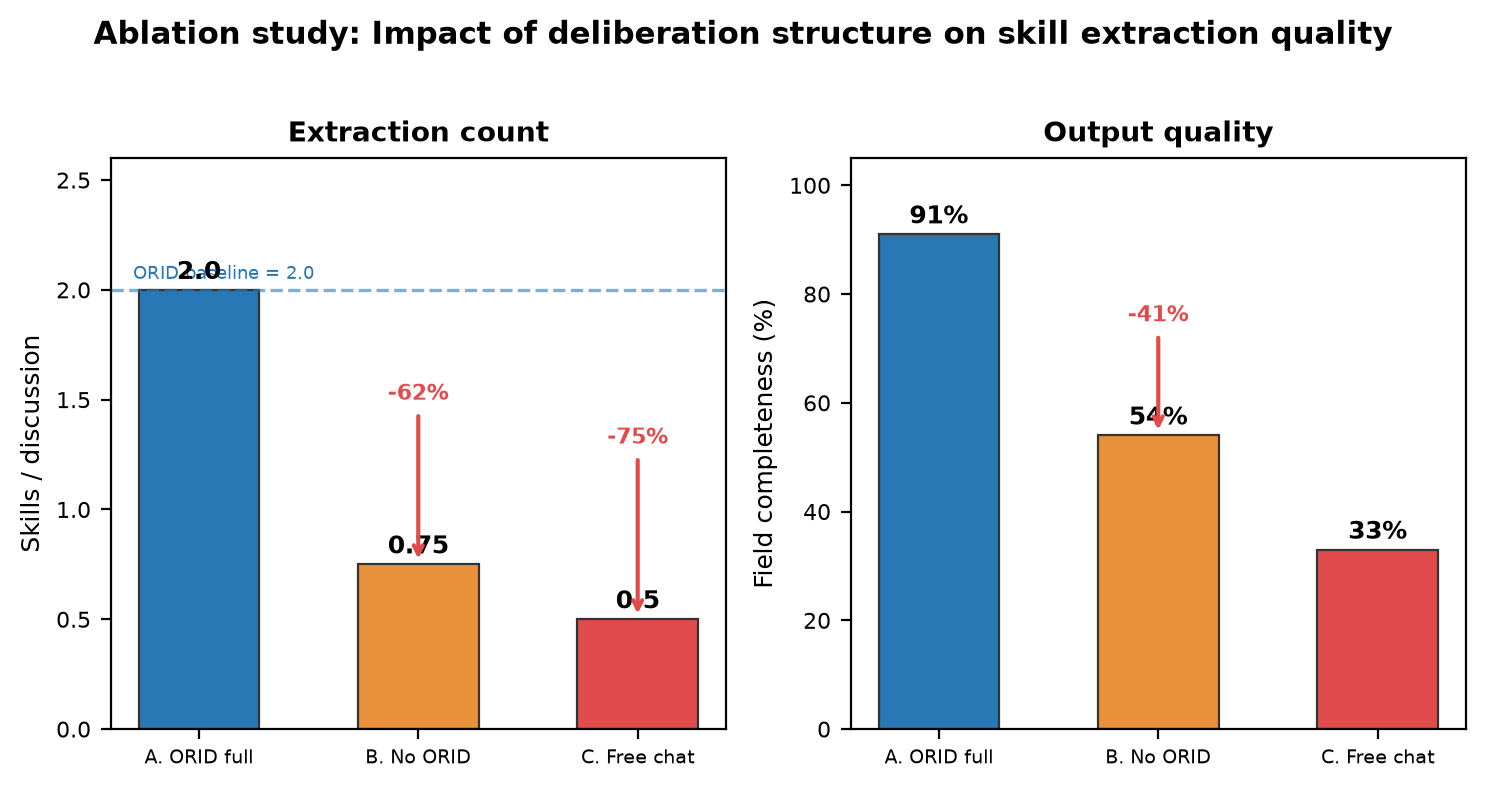
\includegraphics[width=0.95\linewidth]{fig5_ablation.png}
\caption{消融实验——Plaza结构化对知识产出的驱动力：去除ORID议程后，每讨论萃取技能数从2.0骤降至0.75（下降62\%），字段完整性从91\%跌至54\%。没有任何模糊的余地——结构即是力量，无结构便无知识。}
\label{fig:ablation_passionate}
\end{figure}

\begin{figure}[t]
\centering
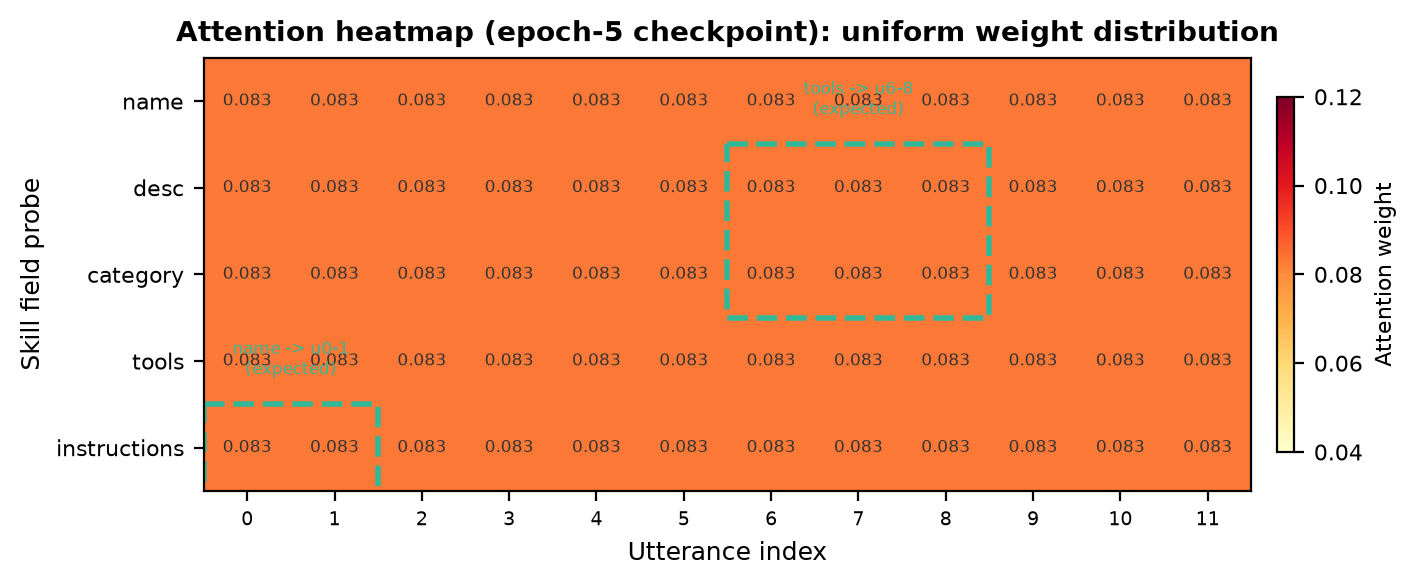
\includegraphics[width=0.95\linewidth]{fig6_attn_heatmap.png}
\caption{注意力热图（epoch-5 checkpoint）：五枚探针在12条话语上的全部注意力都是0.083——完全的均匀分布。模型在"看」，但什么都"没看见"。这是相变前的临界状态——一场等待临界数据注入后的大爆发。绿色虚线框标注了冷启动关键词种子对name和tools探针的预期聚焦区域——一旦相变发生，热图将从这统一的蓝色变为局部燃烧的红色。}
\label{fig:attn_passionate}
\end{figure}

\end{document}
